\documentclass[a4paper,10pt]{article}

\usepackage[utf8x]{inputenc}
\usepackage[french]{babel}
\usepackage{fancyhdr}
\usepackage{graphics}
\usepackage{graphicx}
\usepackage{color}
\usepackage{xcolor}
\usepackage{longtable}
\usepackage{multirow}
\usepackage[pdftex,colorlinks=true,urlcolor=blue]{hyperref}
\usepackage{times}
\usepackage{multicol}
\usepackage{ifthen}
\usepackage{enumitem}
\usepackage[absolute]{textpos}
\usepackage{glossaries} 
\usepackage{fancybox}
\usepackage{floatflt}
\usepackage{wrapfig}
\usepackage{wallpaper}
%opening
\title{}
\author{}
\definecolor{RougeToDo}{rgb}{0.9568,0.0509,0.0392}  % 244 13 10

% \newcommand{\todo}[1] {
%   \ovalbox{
%       \begin{minipage}{2in}
%       \textit{\color{RougeToDo}{#1}}
%       \end{minipage}
%   }
% }

\newcommand{\sidebox}[2]
{
\begin{center}
-----------------------------------------------------------
\end{center}
\begin{center}\textbf{#1}\end{center}
\textit{#2}
\begin{center}
-----------------------------------------------------------
\end{center}
}

\newcommand{\glse}[2]
{
  \newglossaryentry{#1}{name={\texttt{#2}},description={TODO\newline Mentionné p}}
%\include{more/#1}}}
}
%% acronyms, organisations
\glse{fbi}{FBI}
\glse{tlc}{Lindbergh Case}
%% pnjs

\glse{bgw}{Betty Gow}
\glse{ewm}{Evalyn Walsh McLean}

\glse{ctn}{Clyde Tolson}
\glse{ejh}{Edgar J.Hoover}
\glse{jafsie}{Jafsie}
\glse{gms}{Gaston Means}
\glse{wbs}{William Sullivan}
\glse{ams}{Ambrose Morgens}
\glse{clg}{Charles Lingbergh}
\glse{osd}{L'Ordre Esoterique de Dagon de Throg's Neck}
\glse{evk}{Eugene Vander Klei}
\glse{lgt}{L\'{e}on G. Turrou}
\glse{john}{``John''}
\glse{fbiHq}{``Si\`{e}ge du Gouvernement''}

% mythes
\glse{nya}{Nyarlatothep}

% Sources
\glse{sny}{Les Secrets de New York}

\makeglossaries

\begin{document}
\begin{titlepage}


\begin{center}
\vspace{20pt}
% Title
\hrule
\vspace{3pt}
{ \huge \bfseries Lindbergh Case}
\vspace{3pt}
\hrule
\vspace{10pt}
% Upper part of the page
\begin{center}
 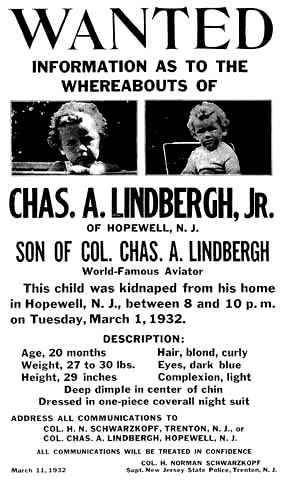
\includegraphics[scale=0.9]{../docs/cover.jpg}
 % cover.jpg: 282x482 pixel, 96dpi, 7.46x12.75 cm, bb=0 0 212 362
\end{center}
\vfill
\hrule
\vspace{3pt}

% Author and supervisor
\begin{minipage}{0.4\textwidth}
\begin{flushleft} \large
\emph{Auteur:}\\
Romain PELISSE
\end{flushleft}
\end{minipage}
\begin{minipage}{0.4\textwidth}
\begin{flushright} \large
\emph{Un scénario pour:} \\
L'Appel de Cthulhu\textcopyright
\end{flushright}
\end{minipage} 
\end{center} 
\end{titlepage}


\begin{abstract}
\textit{\paragraph{}Le \emph{Lindbergh Case} est un scénario pour l'Appel de Cthulhu inspirée par l'enquête du même nom 
sur le \emph{kidnapping} du fils du célèbre aviateur Charles Lindbergh. Prenant le rôle d'investigateurs
spéciaux mandés par le directeur du FBI, le non moins fameux Edgar J. Hoover, les investigateurs auront
l'opportunité de soulever le voile de mystère autour de l'affaire...}
\end{abstract}

\LRCornerWallPaper{0.2}{../artifacts/right-corner-image.png}


\section{Intrigue et contexte}
\subsection{Introduction}
\subsection{Le Lindbergh Case}
\paragraph{} Ce scénario se déroule donc dans le cadre historique du \emph{\gls{tlc}}, comme l'a baptisé le
\gls{fbi}. La déroulement des actions, et l'implications des différents personnages historiques et la chronologie, y est 
autant que possible respecter, ce qui vous permettra de vous référer sans difficultés aux nombreuses sources disponibles
sur le sujet. Une bibliographie et une ``webliographie'' est présente en annexe à cette intention.
\paragraph{} Bien évidement, pour vous faciliter la lecture et la prise en main du scénario, un résumé de l'affaire, du
déroulement des évènements et des personnages clés est présent ci dessous. Si il devrait suffir à mener ce scénario sans
difficultés majeures, se plonger un peu plus en profondeur sur le contexte historique du scénario vous permettra d'apporter
vraisemblablement une touche de profondeur et d'authenticité supplémentaire appréciable à votre narration. Sans compter
évidement qu'une connaissance claire de cette dernière votre permettra plus aisément de répondre aux interrogations de 
vos investigateurs.
\begin{wrapfigure}{r}{60mm}
\ovalbox{
  \scalebox{0.9}{
  \begin{minipage}{2in}
  \textbf{Jouer avec ses investigateurs habituels}
  \tiny{
  \begin{center}------\end{center}
\paragraph{} Si vous souhaitez jouer ce scénario dans le cadre de votre campagne avec les personnages habituels de vos joueurs, il est peu probable
que vous puissiez facilement les transformer subitement en enquêteurs du FBI. Ceci ne forme pas néanmoins pas un réel problème, ni une
réelle difficulté.
\paragraph{} Si \gls{ejh} confie naturellement cette mission à des agents du \gls{fbi}, il peut tout autant la confier à des ``consultants 
externes'' du bureau - vos investigateurs peuvent avoir déjà été engagés par le bureau, probablement pour aider des agents empétré dans une affaire
quelques peu étrange. Que vos investigateurs y ait joués un rôle de démystificateur\footnote{Dévoilant, encore une fois, comme dans tout bon
épisode de \emph{Scoobidoo}, que le fantôme, c'était le directeur du musée.} ou au contraire aient usées de leurs connaissances des abominations
du Mythe de Cthulhu, ils n'en restent pas moins qu'ils ont été chaudement recommandé par des agents du FBI au directeur. 
\paragraph{} Peut être, ont ils aidés \gls{ctn}, le fidèle bras de droit de \gls{ejh} avant qu'il n'accède à un si haut échellons du Bureau. A 
moins qu'il n'est aidé, le numéro 3, Cartha (TODO) dans une affaire embarrasante. Quoiqu'il en soit, les investigateurs sont fortement recommandés
pour leur discernement et leur discrétion au directeur qui opte donc pour les utiliser, plutôt que ses propres agents, diminuant d'autant plus le
risque d'implication du Bureau.
  }
  \end{minipage}
  }
}
\end{wrapfigure}


\subsection{Les Secrets de New York}
\paragraph{} L'action du \gls{tlc} se déroulant essentiellement à New York City, et plus spécifiquement, dans sa banlieue célèbre 
du Bronx, le guide pour l'Appel de Cthulhu \gls{sny} a aussi été une inspiration importante pour ce scénario. Les deux principales
opposants des investigateurs en sont directement extraits:
\begin{itemize}
 \item \gls{ams}, un sorcier plusieurs fois centenaires, mais aussi un riche - mais discret, notable de New York est décrit amplement 
dans le guide \gls{sny}. Il est le ``véritable'' commanditaire du \emph{kidnapping} du jeune fils de \gls{clg} et le démasquer forme 
donc, du point de vue des investigateurs un objectif essentiel.
 \item \gls{osd}, très succintement évoqué dans le guide, joue ici un rôle de ``sous traitant'' pour \gls{ams} s'étant chargé pour 
son compte du \emph{kidnapping}.
\end{itemize}

\begin{wrapfigure}{l}{40mm}
\ovalbox{
  \scalebox{0.9}{
  \begin{minipage}{2in}
  \textbf{Et si les investigateurs ont déjà joué le scénario la Demi Lune ?}
  \begin{center}------\end{center}
  \paragraph{} Ce scénario, inclut dans \gls{sny}, base sa trame sur la découverte et la destruction du sorcier et de son culte 
par les investigateurs. Dans le cas, où vous sohaiteriez jouer ce scénario avec les mêmes investigateurs, il faudra opérer quelques
modifications au scénario:
\begin{itemize}
 \item les pistes du scénario menant à \gls{ams} mèneront à un membre de sa secte, dont les investigateurs pourront se rappeler suite
à leur précédente enquête sur le sinistre sorcier. Si ils avaient réussi à écrouer l'individu, ils se rappeleront que ce membre de la
secte avait réussi à échapper aux poursuites judiciaire, faute de preuves. Notez qu'un membre de la cour suprême ferait un bon remplaçant 
à \gls{ams}, car un tel personnage entrainerait autant de prudence que \gls{ams} chez \gls{ejh}. 
 \item les installations de la Morgens Institude (TODO page du guide) auront été vraisemblablement abandonnées à la suite des investigations
de vos joueurs, il faudra donc relocaliser ces derniers. Le guide \gls{sny} vous aidera dans cette tâche, mais, en guise de suggestion, 
\gls{ams}
  \item Si \gls{ams} n'avait pas survécu à sa rencontre avec vos personnages, il sera de retour pour ce scénarion, réincarné par l'un des survivants
de la secte. Evidament, la réssurection de ce dernier nécessitait de s'emparer du corps, sans éveiller les éventuels autorités, une tâche, où là 
encore, un juge de la Cour Suprême excellerait.
\end{itemize}
  \end{minipage}
  }
}
\end{wrapfigure}

\subsection{Les rêves eugéniques de Ambrose Morgens}

\paragraph{} Comme décrit dans \gls{sny} , \gls{ams} est sorcier aux services de \gls{nya} qui est obséder, depuis maintenant plusieurs
millénaires, par l'amélioration, par transformation relativement radicale, de l'espèce humaine. Les idées eugénistes sont à la mode dans 
les années vingts et l'on discute à tout bout de champs du ``problème'' du mélange des races. C'est ce genre de réflexion qui aboutira en
1924 (TODO, lien date) à la publication du National Immigration Act. Néanmoins, cette mode a beaucoup aidé le sorcier dans ses recherches,
lui apportant entres autres, et jusqu'à la crise de 1929, de nombreux financement.
\paragraph{} Il se sent, avec son comparse \gls{evk}, qu'il considère plus comme un outil qu'un collaborateur, près à réaliser l'ultime transformation, qui aboutira à la création d'une nouvelle espèce, supérieur, de l'homme. Pour réaliser ce dernier pas vers leur succès, ils ont décidés qu'il leur faudrait, en guise de cobaye, un bébé de quelques mois à peine, mais au potentiel génétique de forte qualité. 
\paragraph{} L'idée de \emph{kidnapper} le fils de \gls{clg} leur vint presque naturellement. En effet, \gls{clg} est une sorte de ``super start''
pour l'époque, même si son dégout pour les bains de foules à fini par retourner une partie de l'opinion, frustré de son manque de présence, contre
lui. Néanmoins, pour \gls{ams}, son fils, possédant clairement des gênes de grandeur, aux regards des exploits de son père, est un parfait cobaye
pour réaliser leur prochaine expériences.
\paragraph{} Il reste pour autant encore de réaliser le rapt en lui même, ce qui n'est pas simple, car la célébrité de l'aviateur lui assure la
collaboration de nombreuses forces de polices et agence - comme ça sera le cas, or la secte n'apprécie pas l'idée de risquer d'être découverte
lors de l'enquête qui suivra l'exécution du crime. C'est alors que le sorcier pense à \gls{osd}

\subsection{L'Ordre Esotérique de Dagon de Throg's Neck}

\subsubsection{L'alliance avec Ambrose Morgens}

\paragraph{} Au début des années 1930, \gls{ams} est rentrée en contact avec quelque uns des membres
de l'\gls{osd}, et a commencé avec eux un avantageux commerce. En échange des services de la secte, 
le sorcier leur fournit, sur une base régulière, des \emph{femelles} - comprendre des femmes qu'il a 
kidnappées pour ses propres besoins. Une fois ces dernières rescapés du laboratoire de son comparse, et 
créature, \gls{evk}.

\paragraph{} Néanmoins quand il ne s'agit plus de \emph{kidnapper} quelques jeunes adolescents brillant 
de la haute société New Yorkaise, mais le fils du plus grand héros des états unis (\gls{clg} est une véritable 
icône pour ses comtemporains), \gls{ams} décide d'utiliser le culte comme intermédiaire, sachant que sa 
relation avec eux est très tenue. Le culte ignore qui il est vraiment, car si il préfèrent rencontrer \gls{osd}
en personne, généralement dans les cimettières du Bronx, il prend toujours soin de masquer son visage, comme
sa voie, à l'aide de Magie.

\subsubsection{Profonds et reproduction}

\paragraph{} La communauté de Throg's Neck est essentiellement composée de vieilles familles de pêcheurs, 
qui se sont recyclés en garde maison quand les riches ont transformé, assez brièvement, le village en une
sorte de port de plaisance pour riche désoeuvrés dans les années 20.

\paragraph{} La communauté est entièrement noyauté par \gls{osd}, à l'insu des rares notables de New York qui
fréquente encore le lieu pour son port de plaisance. Une splendide demeure de vacances, situé presque au centre
de la ville est à l'abandon. C'est du moins l'impression qu'ont les visiteurs du port de plaisance quand ils
viennent, à partir du 1er juin. En fait, cette dernière est squatté depuis des années par le culte, et ses 
sous sols abritent les reliques du cultes et sert aussi à dissimuler les jeunes femmes et jeunes hommes 
fournies par \gls{ams}

\paragraph{} Mais que fait \gls{osd} des victimes de \gls{osd} ? Ils les livrent simplement aux profonds, il en 
existe une petite communauté, dégénérescente, au large de New York. Cette dernière, fidèle aux règles de la
reproduction de ces créatures, a connu une brutale chute de la natalité à partir de 1925. En effet, les 
profonds avaient atteint leur population "maximum" et, naturellement, comme ils arrivent souvent pour ces 
créatures, la croissance de leur population s'est donc arrêter. En effet, les Profonds étant immortels, se reproduit
sans arrêt auraient des effets plus que néfaste sur leur communauté.

\paragraph{} Malheureuseument pour eux, les assauts du \gls{fbi}, en 1926 et 1927, sur leurs refuges côtiers\footnote{
Voir la nouvelle de HP Lovecraft \emph{Les Ombres de Innsmouth}.} ont largement semé la panique chez les Profonds. Leur
population a mal survécu au stress, et le réflexes naturellement isolationistes de ces créatures, ont détruit des 
communauté entières. Ainsi, 

\subsection{Déroulement de l'affaire}
\subsubsection{Le kidnapping}
\paragraph{} Le 1 mars 1923, à 20h, la nurse du tout jeune file de \gls{clg}, \gls{bgw}, couche le bébé dans son berceau. Vers 
21h30, \gls{chg} entend un bruit qui lui fait penser que quelques choses est tombé dans la cuisine. A 22h, \gls{bgw} réalise que
le bébé n'est plus dans son berceau. Elle se renseigne auprès de Madame Lindbergh, qui vient de sortir de son bain. Réalisant que
le bébé n'est pas non plus avec sa mère, elle se rend auprès de \gls{clg}, qui était dans la bibliothèque juste en dessus de la
nurserie. 
\paragraph{} \gls{clg} se rend à son tour dans la nurserie et constate la disparition de son fils. Alors qu'il fouille la chambre,
il découvre une enveloppe blanche qui a été laissé sur le radiateur, près de la fenêtre. Il s'empare ensuite de son fils et explore 
la maison à la recherche d'intrus. Dans la demi heure qui suivirent, les forces de police locales sont en route pour la demeure,
comme les médias, et l'avocat de \gls{clg}.
\paragraph{} La police fouille les lieux et trouve rapidement une piste boueuse reliant la fenêtre du jeune enfant à un bosquet
où est dissimulée une échelle bricolé mais astucieusement conçu. Si la criminalistique, déjà à l'époque, aurait permis de retirer
beaucoup plus d'éléments à partir de ces quelques traces, le temps pluvieux et la contamination rapide de la scène du crime, n'a 
pas permis de découvrir plus d'éléments.  
\paragraph{} Le \emph{kidnapping}, bien que réalisé un membre de \gls{osd}, n'a fait appel à aucune sorte de magie ou de créatures
du Mythe de Cthulhu. Le cultiste habile a juste pensé à bien masquer ses empreintes dans le sol, une fois l'échelle abandonnée et 
à droguer légèrement le jeune bébé pour s'assurer qu'il ne crie pas pendant sa fuite. Un comparse, aussi membre du culte, l'attendait
non loin dans une voiture.
\subsection{Tout le monde s'emmêle}
\paragraph{} La notoriété de \gls{clg} a effet probablement très désatreux sur l'affaire. Dans la nuit même, \gls{ejh}, réveillé exprès
par un de ses assistants ayant appris la nouvelle, appelle \gls{clg} pour l'informer que le Bureau se tient près à assister l'enquête.
Dans le même temps, \gls{wbs}, le fondateur de la future OSS et de la CIA, arrive et offre aussi ses services. Bientôt, la situation
remonte jusqu'au bureau du président Roosevelt...
\subsection{Gaston Means et la jeune héritière}
 


%http://en.wikipedia.org/wiki/Evalyn\_Walsh\_McLean

%http://en.wikipedia.org/wiki/Gaston\_Means

%http://www.charleslindbergh.com/

% http://news.google.com/newspapers?id=cXAbAAAAIBAJ&sjid=WEsEAAAAIBAJ&dq=gaston%20means&pg=3047%2C5884625
% http://news.google.com/newspapers?id=cXAbAAAAIBAJ\&sjid=WEsEAAAAIBAJ\&dq=gaston\%20means&pg=3047\%2C5884625

% http://en.wikipedia.org/wiki/Saint_Raymond's_Cemetery,_Bronx

% http://en.wikipedia.org/wiki/Virginia_Hall

% http://www.flickr.com/photos/neatnessdotcom/1564083369/sizes/l/

\subsection{timing}

- \gls{ejh} enterre l'affaire dès la découverte du jeune Lindberg le 12 mai:

On May 12, 1932, delivery truck driver William Allen pulled his truck to the side of a road about 4.5 miles (7.2 km) from the Lindbergh home. He went to a grove of trees to relieve himself, and there he discovered the corpse of a toddler

\pagebreak
\section{Arrestation de Gaston Means}
\subsection{Briefing avec Leon Turrou}

\paragraph{} Pour les investigateurs, le scénario commence par une rencontre avec \gls{lgt}, dans le bureau qu'il occupe dans 
un commissariat de New York City. Sommairement, l'agent les informe que le Bureau vient de les réaffecter en renfort à sa
\emph{task force} sur le \emph{Lindberg Case}. Leur arrivée est appréciable, car il y a beaucoup à faire, mais le dossier 
est vaste, il va être difficile de vite les mettre à niveau. ``En conséquence, le Directeur et moi avons commencé par confier
un tâche ne nécessitant pas une connaissance profonde du dossier : l'arrestation de \gls{gms} !''.

\begin{wrapfigure}{r}{50mm}
\begin{center}
 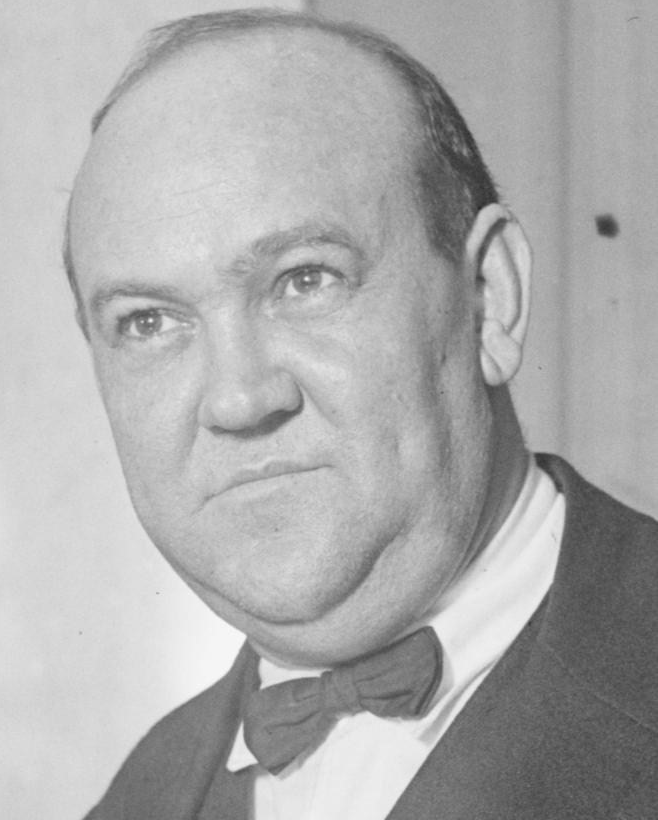
\includegraphics[width=40mm]{../pnjs/gaston-means-1924.png}
\end{center}
\caption{Gaston Means - 1924}
\end{wrapfigure}

\paragraph{} \gls{lgt} rappel sommairement le ``brillant'' parcours de \gls{gms} au sein du \gls{fbi} et décris sommairement
comment il a profité de l'affaire Lindbergh pour escroquer la jeune héritière. Il ajoute qu'il est fort content que cet 
ultime bévue permette enfin au Bureau de placer cet ancien collaborateur plus qu'embarassant sous les barreaux.

\paragraph{} Il souligne de manière un peu condescendante que l'arrestation est une opération simple que les investigateurs
seront à même de réaliser sans maitriser entièrement le dossier. Une fois l'odieux personnage remis au plus proche commissariat,
les investigateurs pourront rejoindre la ``task force'' dédié à l'affaire Lindbergh.

\paragraph{} ``Ah, et un dernier point, le Directeur (\gls{ejh}) souhaite que vous profitiez de votre passage à Washingthon, 
pour le rencontrer, après l'arrestation \gls{gms}. Ca sera tout, merci.''. L'agent \gls{lgt} les remercier promptement. Arrivée 
à ce stade, il est important de faire comprendre à vos agents, que la dernière remarque de \gls{lgt} leur fait l'effet d'une 
bombe. Rencontrer en personne \gls{ejh} peut s'avérer fatal pour la carrière de tout agent du Bureau, et l'homme est connu pour
son caractère particuliers et ses réactions surprenantes.

\paragraph{} Avec un test de psychologie sur \gls{lgt}, vos agents pourront aussi noter que tout le discours de ce dernier est 
quelques peu étranges. Il les acceuille de haut et les considérant comme des membres, mineurs, de son équipe, à qui il confie une
tâche simple pour commencer. Néanmoins, sa dernière requête, la rencontre avec \gls{ejh} laisse présager que leurs rôles sera 
beaucoup plus cruciale.

\paragraph{} En fait, \gls{lgt} essaye de sauver les apparences. \gls{ejh} la contacter la veille pour lui demander de réunir
les investigateurs, de les briefer sur l'affaire et de leur confier l'arrestation de \gls{gms}. Il n'a jamais placé les agents
sous sa juridiction et il ne compte pas le faire. En se positionnant, vis à vis d'eux, comme le SAC (\emph{Special Agent in Charge}
du dossier, \gls{lgt} espère les impressionner assez pour qu'il se place tout naturellement sous son autorité, quelques soit la
mission relative à l'affaire que leur confiera le Directeur. Son comportement n'est, comme souvent dans le Bureau, qu'une simple
manoeuvre politique.

\paragraph{} Si \gls{lgt} craint pour sa position de SAC de l'affaire, il n'est pas dans les projets du Directeur de le remplacer.
En fait, \gls{ejh} entends juste confier aux investigateurs une mission totalement secrète, même si elle est liée à l'affaire
Lindbergh, il entend bien garder son SAC dans l'obscurité la plus totale à ce sujet...

\paragraph{} Bien que \gls{lgt} essaye de clore rapidement l'entretien, rappelant aux agents qu'ils ont longue route avant la capitale
et qu'ils doivent arrêter \gls{gms} au plus tôt, le SAC acceptera de répondre à leur question. Il n'a aucun idée de ce que pourra
être leurs prochaines tâches dans le cadre de l'enquête et il reste donc évasif (``Il y a beaucoup à faire et le dossier évolue
rapidement, nous ferons le point à votre retour''). Il ignore aussi pourquoi \gls{ejh} les a choisi eux plus que d'autres pour arrêter 
\gls{gms}. Interroger sur ce point, il sera presque honnête : ``Le Directeur et moi estimons qu'il faut rapidement arrêter cet 
individu et j'ai besoin de toutes mes ressources actuelles à New York''.

\paragraph{} En fait, les choses utiles que les agents peuvent obtenir de lui, c'est les réponses à toutes leur questions sur 
l'enquête en cours et la situation actuelle. En fait, cette séquence est principalement là pour vous permettre de ``briefer'' les PJs
sur le dossier de manière plus interactive qu'un long monologue sur le sujet. 

\subsection{L'arrestation de l'incroyable Gaston Means}

\paragraph{} A la fin de son \emph{briefing}, \gls{lgt} remet le mandat d'arrêt pour \gls{gms}, obtenue auprès d'un juge de New York,
et les clés d'un véhicule de fonction du Bureau, pour se rendre à la capitale. Il y a près de 250 \emph{miles} qui sépare la grande
Pomme de Washington DC, et si on peut aujourd'hui réalise ce trajet en 5h, à l'époque la vitesse des véhicules et la qualité des 
infrastructures ne permettaient vraisemblablement pas de faire le trajet en moins de 8h - et encore avec un minimum de pause. 

\paragraph{} En étant libéré entre 9h et 10h du bureau de \gls{lgt}, les Agents arriveront donc à la capitale, à la résidence de 
\gls{gms} entre 17h et 19h. La rencontre avec \gls{ejh} se déroulera donc ensuite, mais les Agents savent que le Directeur sera
toujours dans son bureau, près à les recevoir.

\paragraph{} \gls{gms} est chez lui et il ne s'attend pas à l'arrivée des Agents ni à son arrestation. Il ne soupçonne pas que la
jeune héritière les dénoncer et même si c'est le cas il s'imagine encore que le Bureau, son ancien employeur le protégera. \gls{gms}
se croit encore du temps du président Harding, où la corruption et l'abus de pouvoir caractériser plus les agents du \gls{fbi} que 
l'image de ``super flic'' en pardessus que nous avons aujourd'hui d'eux. 

\paragraph{} Quand les Agents viendront l'arrêter, il se comportera comme un innocent injustement accâblé, insistant sur le fait 
qu'il a remis l'argent de la jeune héritière à l'un de ses collaborateurs. Même si ils étaient assez naïf pour croire le mythomane,
les Agents ne peuvent simplement pas faire autrement que de l'arrêter. Alors que les PJs ne croit pas à ses régimiades, et ne semble
pas réagir à son appel à la ``camaraderie entre personnes du Bureau'', il finit par jouer sa dernière carte.

\paragraph{} ``Hoover fait une grave erreur en m'arrêtant ! Sans moi, le Bureau ne retrouvera jamais le petit Lindbergh en vie ! Vous 
êtes entrain de sacrifier votre dernière espoir de le retrouver pour satisfaire les frasques d'une jeune riche héritière déjantée !''.
\gls{gms} refusera d'être plus clair à ce sujet. Il sait que si il révèle quoique soit maintenant, il n'aura plus aucune carte à jouer
en prison.

\paragraph{} Néanmoins, les Agents ont une carte dans leur manche. Le mandat d'arrêt comprend aussi un mandat de perquisition qui leur
permet de fouiller les lieux. Le juge avait remis ce mandat plus pour permettre aux agents de fouiller la résidence de \gls{gms} au cas
où celui ci est pris la fuite. Ils peuvent néanmoins s'en servir, même si \gls{gms} s'est révélé plus collaboratif qu'escompté.

\paragraph{} Lorsqu'ils fouilleront la demeure de l'escroc, les Agents ne trouveront qu'un seul élément relatif à l'affaire Lindbergh -
mais n'hésitez pas à y placer quelques autres fausses postes. Il s'agit d'une simple carte de visite, du \gls{plc}, glissé sous un coin
du grand buvard, indemne de toute trace d'encre, qui recouvre le bureau de \gls{gms}. Cette carte de visite représente le seul lien 
concret entre l'ancien agent et l'affaire. 

\paragraph{} \gls{plc} lui a remis sa carte en mains propres, après l'avoir rencontré en compagnie de lajeune héritière, \gls{ewm}. Se 
servant du crédit de la demoiselle, \gls{gms} s'est présenté comme un enquêteur spéciale, littéralement en charge secrètement de la 
disparition du petit Lindbergh. \gls{plc} est tombé dans le panneau et lui a immédiatement fait part de ses soupçons envers \gls{ams}, 
qu'il connait bien parce qu'il partage ses idées sur l'eugénisme.

\paragraph{} En évoquant avec \gls{ams} l'affaire Lindbergh, lors d'un diner mondain, le riche New Yorkais lui a fait une réponse sybbiline
sur le devenir du jeune bébé et la perte, en terme génétique, que représentait sa disparition. \gls{plc} a eu du flair (01 sur un jet de 
psychologie !) et a compris que le millionnaire en savait plus long qu'il ne le disait sur cette affaire.

\paragraph{} Depuis, \gls{plc} soupçonne fortement \gls{ams} d'être impliqué par un moyen ou un autre dans cette histoire, mais il ne
savait pas quoi faire. Sa rencontre avec \gls{gms} lui a offert un moyen de soulager sa conscience, même si, malheureusement, \gls{gms} ne 
sera pas quoi faire de cette information - si ce n'est l'utiliser comme un joker dans la dernière chance pour tenter d'échapper encore une
fois à la justice.

\paragraph{} Malheureusement pour le pauvre \gls{plc}, \gls{ams} n'a pas survécu pendant plusieurs siècle sans un sens aïgu de la paranoïa.
Il a bien senti lors de la discussion avec lui qu'il en avait d'une certaine manière beaucoup trop dit. Il a rapidement fait surveiller le
professeur, et, peu après sa rencontre avec \gls{gms}, le sorcier a décidé qu'il était plus prudent de se débarasser de lui, plutôt que de
risquer de le voir l'impliquer, même sans preuve, dans la disparition du petit Lindbergh. \gls{ams} est conscient que tout les forces de 
polices ou agences gouvernementable impliqué dans les investigations sont suffisament déséspérés pour l'investiguer lui, en détail, malgré
ses relations. Et comme tout cultiste, il sait que si on examine ses activités de manière trop minitieuse, on ne serait manqué toutes les
choses qu'il cherche à cacher à tout prix...

\subsection{Rencontre avec le Directeur}

\paragraph{} Une fois \gls{gms} arrêté et remis au plus proche poste de Police,les agents sont peuvent enfin se précipiter à leur rendez 
avec \gls{ejh}. Même, si le directeur n'est au contrôle du Bureau que depuis le milieu des années 20, sa ``légende'' au sein de ce dernier
est déjà en place. Les investigateurs savent qu'ils doivent la jouer fine avec ce dernier, car, si il lui déblaise, leur carrière sera
fini net. Et même si jamais, les investigateurs n'avaient que faire de leur carrière, il est important de leur signaler que la capacité
de ``nuissance'' du Directeur dépasse largement les limites du \gls{fbi}.\footnote{Pour donner du relief à cette scène, le meneur de jeu
est invité à se renseigner quelques peu sur l'étonnant personnage qu'était \gls{ejh}, pour lui en faciliter l'interprétation}.

\paragraph{} Déjà fidèle à son poste, c'est la secrétaire personnelle du Directeur, \href{http://en.wikipedia.org/wiki/Helen\_Gandy}{Helen Gandy}
qui, malgré l'heure tardive de leur arrivées, acceuille les investigateurs. Elle les salue brièvement, et se lève pour se rendre dans le 
bureau \gls{ejh} pour lui signifier leur présence. Elle en resort quelques instants plus tards, pour les prier de rentrer.

\paragraph{} A peine les investigateurs sont ils rentrés dans le bureau, plongé dans une semi obscurité - la seule source de lumière est 
la lampe posé sur le bureau du directeur, que la secrétaire referme derrière eux la porte. Il faut quelques secondes pour leurs yeux s'habituent 
a lumière tamisée de la pièce. Alors que leur vue s'accomode, ils constatent que le directeur les regarde en silence, en les invitant d'une
main à s'assoir sur les quelques sièges installés, en contre bas, devant son bureau.

\paragraph{} Sans transition, il leur demande si l'arrestation de \gls{gms} s'est bien déroulé. Le directeur écoute les calmement, sans faire 
de commentaire, le récit des personnages. Néanmoins, il ne peut contenir un sourire de satisfaction, au fur et à mesure de leur récit. Une fois
leur rapport terminé, il les félicite pour cette affaire ``rondement menée''. Avec un test de psychologie, les personnages pourront comprendre
que ces félicitations gratuites ne sont due que à la bonne humeur du directeur, qui est très satisfait de voir enfin \gls{gms} derrière les 
barreaux.

\paragraph{} Après ce petit moment de joie, \gls{ejh} il reprend immédiatement un ton très grave : ``Messieurs, je pense que la presse et l'agent
spécial \gls{lgt} vous permettent d'avoir un vue à peu près complète de l'affaire Lindbergh, à ce jour. Il y a néanmoins une élément nouveau qui 
ne vous a pas encore été transmis''. Le directeur leur résume alors succintement l'implication de \gls{jafsie}, sans cacher son irritation autant
au sujet du vieux professeur que des choix malheureux de \gls{clg}. Il conclu son récit en leur annonçant que ce soir, le vieux professeur et
 \gls{john} doivent de nouveau se rencontrer, pour transmettre la payement de la rançon. A la demande express de \gls{clg}, aucune force de police
ou agence gouvernementale ne doit interférer avec cette opération.

\paragraph{} ``Messieurs, après une longue réflexion, j'ai décidé de prendre le risque de ne pas respecter les demandes de \gls{clg}, qui j'estime
dans ce cas sont déraisonnables et frise l'obstruction à une investigation fédérale !'', une manière, comme une autre, de légitimer une opération
clairement à la limite de la légalité. \gls{ejh} leur explique ensuite qu'il les a donc choisi pour prendre en charge cette mission, car il sait
qu'ils savent être discret, et la discrétion est la clé de l'opération. ``En effet, comprenez immédiatement que si vos agissements compromettaient
le sauvetage du jeune Lindbergh, le Bureau serait très \emph{embarassé}.'', et comme le savent tout agent, \emph{embarasser} le Bureau, signifie,
au moins, la fin de sa carrière, et probablementle début de beaucoup d'ennui généré par \gls{ejh}.

\paragraph{} Les investigateurs, qui ont rencontrés \gls{lgt} à New York, réalise qu'il n'a pas le profil pour ce genre d'opération quasi illicite.
Entre autre, ils comprennent aisément aussi que le choix s'est porté sur eux, car ils n'ont pour 
l'instant aucun rapport avec l'équipe associée à l'Affaire Lindbergh.

\paragraph{} La mission des investigateurs en tant que telle consiste donc à suivre le plus discrètement possible \gls{jafsie} jusqu'au lieu de son
entretien avec son contact parmi les prétendus kidnappeurs, \gls{john}. Ils devront observer, sans intervenir, l'échange et suivre ensuite le 
kidnappeur et tenter d'assurer le retour sain et sauf du bébé. Attention aussi, ils ne doivent pas non plus, par leurs agissements, compromettre 
la manoeuvre de \gls{clg}. ``Si vous avez l'impression que les kidnappeurs sont près à remettre l'enfant en échange de leur rançon, surtout 
n'interférez pas. Votre mission consistera simplement dans ce cas, à regrouper le plus possible d'informations, pour assurer l'arrestation des
kidnappeurs par la suite...''

\paragraph{} \gls{ejh} prend le temps, autant que nécessaire, pour répondre aux questions des investigateurs. Il en profitera à chaque fois
pour leur rappeler l'aspect délicat de leur mission et aussi qu'ils ne doivent en aucun cas \emph{embarasser} le Bureau. Après ce long 
\emph{briefing}, les investigateurs quitteront vraimsemblablement le quartier général du bureau aux alentours de minuit. Ils ne disposent que
de peu de temps pour dormir avant de reprendre la route, pour être à temps à New York, demain soir. Officiellement, \gls{ejh} a signé un document affirmant
qu'ils sont à Washington DC, pour s'occuper des suites de l'arrestation de \gls{gms}...
\pagebreak
\section{Scène 2: Mission secret pour le Bureau d'Investigation}

\subsection{Au chat et à la souris, à travers Manhattan}

\paragraph{} Equippé d'une seule voiture de fonction, un banal Fort T, avec dans le coffre un attirail de déguisement, les 
agents arrivent devant la demeure de \gls{jafsie}, après une route épuisante de près de 6h ou 7h\footnote{Test de Conduite pour 
le pilote, sinon -1 point de vie, causé par la fatigue à tous les passages}. Ils arrivent juste à temps, le vieux monsieur, 
clairement nerveux, mais décidé, vérouille sa porte et se prépare à partir.



\subsection{Le Cimetière Saint Raymond}

\paragraph{} Après une délicate filature de \gls{jafsie}, qui a été baladé dans presque tout Manhattan, avant d'être redirigé 
vers le Bronx, les investigateurs arrivent, à quelques centaines de mètres derrière le professeur à la retraite, en vue du 
Cimetière Saint Raymond. Sachant que le premier rendez vous avec les prétendus kidnappeurs a eu lieu dans le cimetière de Woodland,
les agents sentent intuitivement qu'ils parviennent enfin au lieu du rendez vous.

\paragraph{} Pénétrer dans le cimetière à la suite du vieux homme est moins évident que la filature, pourtant déjà peu aisé, qui
les a conduit ici. En effet, la zone est déserte, et \gls{jafsie} a fait déjà un beaucoup infernale, en faisant grincé la porte du 
cimetière. Si quelqu'uns surveille les lieux, suivre, l'air de rien, le vieux professeur ne passera pas inaperçu. 

\paragraph{} Heureusement, même si les investigateurs l'ignorent, la secte n'a rien mis en oeuvre pour surveiller l'arrivée de 
leur intermédiaire. Le vieux professeur ayant respecté les règles du jeux lors du premier rendez vous, ils sont donc désormais un 
peu moins méfiant.

\paragraph{} Quelques soient le stratagème de vos joueurs, leurs personnages devraient arrivées, peu après \gls{jafsie}, au coeur 
du cimetière, et ils ont trouveront refuge derrière une pierre tombale, ironiquement celle d'un Mafiosi mort il y a peu - Joe Cataria, 
pour observer l'échange. Quelques instants après leur arrivée, une église du Bronx sonne au loin minuit - comme quoi ce n'est pas toujours
un cliché, quand émerge de la partie Ouest du cimetière, très boisé, une silouhette. \gls{john}, le contact de \gls{jafsie} vient de 
faire son apparition.

\paragraph{} Tremblant, le vieil homme explique qu'ils n'ont pu réunir que 50 000\$, mais sous interlocuteur ne bronche pas et accepte 
l'argent et lui remet une note lui indiquant que le bébé est sain et sauf à bord d'un bateau, le \emph{Nelly}, à quai dans 
\href{http://en.wikipedia.org/wiki/Martha\%27s\_Vineyard}{Martha's Vineyard}. \gls{jafsie} court prévenir \gls{clg}, qui, lorsqu'ils ne 
trouveront pas le \emph{Nelly}, ira jusqu'à survoler la baie pour tenter de débusquer les kidnappeurs.

\paragraph{} Mais pour les investigateurs, le temps est venu d'honorer la mission secrète que leur a confié \gls{ejh}, suivre \gls{john} et
résoudre l'affaire. Une fois la transaction effectué, \gls{john} regarde le veil homme repartir au pas de course quelques instants, avant 
de lui même se replier vers la même partie boisée du cimetière d'où il a émergé.

\begin{figure}[h]
 \begin{center}
  \includegraphics[scale=0.5]{../handouts/a-la-poursuite-des-profonds-nb.jpg}
  \end{center}
\caption{A la poursuite de ``John''}
\end{figure}

\paragraph{} TODO: Distance / temps sur google maps

\subsection{Retour à la baie de Huson}

\paragraph{} Selon leur discrétion, les agents effectueront une filature, assez complexe, nécessitant quatre jets réussi de Discrétion :
\begin{itemize}
 \fltitem{un pour sortir du cimetière, sans se faire repérer par leur cible ;}
 \fltitem{ un autre pour traverser la Hutchison River Parkway - loin d'être une 4 voies d'aujourd'hui à l'époque et peu fréquenté à cette heure,
 toujours sans se faire voir ;} 
 \fltitem{ un troisième jet pour ne pas se faire repérer en traversant les maisons  entre Rohr Pl. et Senger Pl ;}
 \fltitem{ et enfin un ultime jet pour naviguer dans les entrepôt à poissons, dégageant une odeur plus que nauséabonde.}
\end{itemize}



\paragraph{} A chaque fois qu'un agent rate son jet de discrétion, \gls{john} peut tenter un test de Vigilance (il a 40\%). Si il réussit, il 
repère les agents et panique : il sort son arme à feu (TODO, 30\%), et effectue un \emph{tir de barrage} pour couvrir sa fuite, maintenant au 
pas de courses, vers le barque qui l'attend près des entrepôt.

\subsection{Abattre John}


\subsection{Perdre sa piste}

\paragraph{} Dans le cimetière, ils verront au moins vers où il aller , donc, reflexes de flics assermentés, ils pourront réveiller et interroger les 
habitants des maisons situés entre Rohr Pl. et Senger Pl. Après quelques maisons, un vieil homme, aussi alcoolic qu'insomniaque, aura vu la
silouhette de la \gls{john} se dirigeant vers les entrepots.

\paragraph{} De là, les agents pour répérer (Trouver Objet Caché) la piste boueuse du suspect et la suivre (Suivre une Piste) jusqu'au bord de 
l'eau.

\subsection{Suivre sa piste}

\paragraph{} Si les agents le suivent sans se faire remarquer, ils le verront monter à bord d'une petit barque, qu'il avait discrètement caché dans les 
arbres. \gls{john} jete le lourd sac de toile noire dans lequel il a placé les 50000\$ remis par\gls{jafsie}, et, le plus silencieusement possible, 
s'engage, à l'aide de rame s'engage sur le \href{http://en.wikipedia.org/wiki/Westchester\_Creek}{Westchester Creek}.

\paragraph{} Si ils suspectent leur présence (plusieurs test de discrétion raté du coté des agents, sans succès de sa part pour les repérer), il 
s'éloignera de la cote, mais se rapprochera de nouveau dès qu'il approchera trop de Clason's Point\footnote{Voir les 
\href{http://www.tentacules.net/index.php?id=1180}{Secrets de New York} pour en savoir plus sur Clason's Point et pourquoi un membre de \gls{osd}
se méfie naturellement de cet endroit}. 

\paragraph{} Sa prise distance lui aura été fortement inutile, les agents ne le perdront pas de vue, malgré l'obscurité\footnote{La nuit du 2 mai 1932 n'était 
qu'à \href{www.moonconnection.com/moon_phases_calendar.phtml}{3 nuits d'écart} de la nouvelle lune.}, et cette manoeuvre lui donnera l'impression erronée
qu'il a semet ses poursuivants.


\begin{wrapfigure}{r}{60mm}
\begin{center}
 \includegraphics[scale=0.2]{../handouts/westchester-creek-river.png}
\end{center}
\caption{Westchester Creek River}
\end{wrapfigure}


% bridge : www.panoramio.com/photo/29343659

\paragraph{} Suivre l'esquif alors que \gls{john} canote n'est pas très difficile, mais, alors plus il descend la rivière, plus les alentours deviennent 
relativement rural pour la région de New York. Les agents longent une rivière, caché par quelques arbres, au loin, on peut distinguer la route XXX
et le pont \href{http://en.wikipedia.org/wiki/Bronx–Whitestone\_Bridge}{Whitestone Bridge}, mais aucune voiture n'y circule à cette heure ci et 
force est d'admettre que le grand ouvrage de métal est plutôt lugubre vu d'ici.

\paragraph{} A l'exception du remoud de l'eau et de quelques hulement nocturne, le lieu est désert et semble presque sauvage. La fatigue et la 
tension de la filature continue de jouer des tours aux investigateurs qui, si ils ratent un test de SAN - gardez la caractéristique testé secrète, commence à
distinguer dans les ombres comme des silouettes, nombreuses et que vaguement humaines, qui semblent les observer.

\subsection{Rendez vous sous le Whitestone Bridge}


\begin{wrapfigure}{r}{65mm}
\begin{center}
 \includegraphics[width=64mm]{../handouts/bridge.jpg}
\end{center}
\caption{Whitestone Bridge}
\end{wrapfigure}

\paragraph{} Une fois le pont atteint, \gls{john} s'amarre sous le premier pylone, à 20 mètres de la rive et attend. Rapidement, un petit bateau 
de pêche apparait, le \emph{Nelly} que les investigateurs auront peut être remarqué lors de leur filature de \gls{jafsie} à travers Manhattan. Le
navire de pêche dispose de plusieurs sources de lumière, sous la forme de lampe-tempête accroché ici et là, ce qui permet aux agents d'observer la
scène de loin, avec les jumelles qu'ils auront bien évidemment penser à prendre.

\paragraph{} L'échange sera rapide, \gls{john} remet le sac noir contenant l'argent à un vieux marin barbu, et il se remet en route, toujours plus 
vers le sud. Il rentre chez lui, une maison délabré sur la rive de l'Hudson, dans le quartier de Throg's Neck, les investigateurs peuvent aisément 
continuer à lui suivre si ils le désirent.

\paragraph{} Alors que \gls{john} s'éloigne, le capitaine du Nelly disparait dans son bateau avec le sac noir. Il ressort rapidement avec un lourd
filet de pêche sur le dos. A l'aide d'un jet de Trouver Object Caché, les investigateurs observent la scène que le contenu du filet de pêche semble
se débattre !

\paragraph{} Le vieux marin jete son bardas à l'eau et dans la foulé relance son moteur pour repartir aussi en direction de Throg Neck. Si les 
investigateurs veulent sauver la pauvre femme - une des victimes de \gls{ams} gentillement donner à \gls{osd}, il ne disposent que de peu de temps. Tout investigateurs 
se lançant dans une tentative de sauvetage doit réussir près de 3 jet d'Athlétisme, en tant que Natation, pour arriver assez rapidement, pour sortir
la jeune femme de l'eau.

\paragraph{} Si l'agent ne réussit pas tout ses jets de dés, il ne peut que ramener le corps noyé de la pauvre femme - et encore seulement si il réussit
un test de Puissance pour soulever la frêle créature et le lourd filet de pêche. Avant de tenter la ramener à bon port, il ou ils devront aussi
découper le filet de pêche, assez lourd, qui leur rendrait la tâche impossible. 

\paragraph{} Un autre élément, bien plus effrayant, s'opposera au sauvetage de la jeune femme : un Profond. Le vieux marin n'a pas jeté la pauvre
demoiselle juste pour s'en débarasser, mais pour l'offrir aux Profonds. Une de ses créatures attendait donc sous le pont pour s'emparer d'elle - et
lui jeter un sort permet à la jeune femme de survivre à la noyade. 

\paragraph{} Si les investigateurs interviennent, le Profond, qui comme la plupart de ses comparses évitent la confrontation directe avec les humains,
essayera juste d'attraper sa \emph{promise} et la tirer vers les profondeurs. Une fois que les investigateurs auront ramené la demoiselle à la surface
et essayeront de la libérer de son filet de pêche - action auquelle elle n'opposera ni résistance ni assistance, elle est déjà inconsciente, le Profond
se glisse entre eux et tire subitement sur le filet de pêche pour la faire replonger.

% \begin{wrapfigure}{l}{60mm}
% \ovalbox{
%   \scalebox{0.9}{
%   \begin{minipage}{2in}
%   \textbf{Et si les investigateurs n'assistent pas à l'échange ?}
%   \begin{center}------\end{center}
%   \paragraph{} Dans ce cas, le cadavre de la jeune femme, qui n'aurait pas survécu à la noyade
%   malgré le sort du Profond, réapparaitra le lendemain, non loin de là. Comme les agents auront très probablement rapporté leur escapades dans le
%   Bronx à \gls{ejh}, ce dernier ne manquera pas de faire le lien - ses assistants ont reçu ordre, juste après le rapport des investigateurs de lui 
%   signaler tout rapport ou évènement étranges à New York et dans les environs. Néanmoins, l'information ne parviendra pas exactement au \gls{fbiHq},
%   et les investigateurs n'auront vent de ceci que la nuit d'après, soit le 3 mai.
%   \end{minipage}
%   }
% }
% \end{wrapfigure}

\sidebox{Et si les investigateurs n'assistent pas à l'échange ?}{
\paragraph{} Dans ce cas, le cadavre de la jeune femme, qui n'aurait pas survécu à la noyade
malgré le sort du Profond, réapparaitra le lendemain, non loin de là. Comme les agents auront 
très probablement rapporté leur escapades dans le Bronx à \gls{ejh}, ce dernier ne manquera pas 
de faire le lien - ses assistants ont reçu ordre, juste après le rapport des investigateurs de 
lui signaler tout rapport ou évènement étranges à New York et dans les environs. Néanmoins, 
l'information ne parviendra pas exactement au \gls{fbiHq}, et les investigateurs n'auront vent de
ceci que la nuit d'après, soit le 3 mai.
}

\paragraph{} Avec un test de Vigilance réussit, les investigateurs pourront opposer un test de Puissance face au Profond et pourront peut être l'empêcher
de s'emparer de sa victime. En outre, ils pourront percevoir que \textit{quelque chose} se déplace sous eux (Au cas où vos agents se sentent
grisés de porter un badge du \textit{Bureau of Investigation} et décide de faire un \textit{carton}, rappelez leur l'effet regretable de l'eau
sur la poudre...).

\paragraph{} Le Profond n'insistera pas longtemps et cherchera à tout prix à éviter la confrontation, si ceux deux premières tentatives échouent ou
si les investigateurs arrivent rapidement à libérer la jeune femme du filet de pêche, il abandonne et s'enfonce dans le fond des eaux, pour rejoindre
l'Hudson puis l'océan.

\pagebreak
\section{Rapport à Edgar J. Hoover et suite de l'investigation}

\paragraph{} 

\subsubsection{Enquêter sur ``John''}

\paragraph{} Si les agents ont décidés de suivre \gls{john} jusqu'à son domicile, ils savent désormais qu'il habite une vieille maisonnette, près
de l'\emph{Hudson River}, dans \emph{Throg's Neck}

\subsubsection{Le Nelly et son étrange capitaine}

\subsubsection{L'Ordre Esotérique et Violet Sharpe}

% { Culte a emprise sur Violet Sharpe}

\subsection{La victime, Sadie Newton}

\subsection{Ce que sait Gaston Means}

\begin{itemize}
 \item brillante étudiante des cours du soir à l'Université de la ville de New York (136ième à 140ième rue / Amsterdam Avenue)
 \item issue de la \emph{New York nobility}
 \item disparue le 4 janvier 
\end{itemize}

\pagebreak
\section{Annexes}
\subsection{Personnages, lieux et organisations}
\glossarystyle{super}
\printglossaries
\subsection{Calendrier de 1932}
\begin{center}
 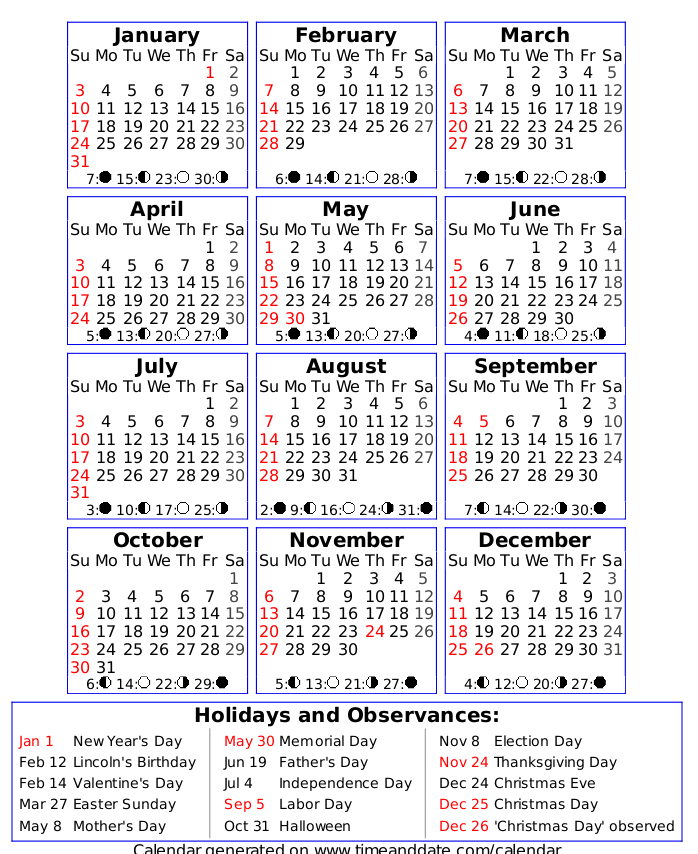
\includegraphics[scale=0.5]{../timeline/1932.png}
 % 1932.pdf: 0x0 pixel, -107374175dpi, 0.00x0.00 cm, bb=
\end{center}


\end{document}
